\documentclass[a4paper,12pt,twoside]{article}

\usepackage[english]{babel}						% language package
\usepackage[utf8]{inputenc}						% input character encoding
\usepackage[T1]{fontenc}							% output character encoding
\usepackage{natbib}								% bibliography package
\usepackage{graphicx}							% for including figures
\usepackage{amsmath, amssymb}					% math environment
\usepackage[
		colorlinks,
		bookmarks=false,
		linkcolor=blue,
		urlcolor=blue,
		citecolor=blue]{hyperref} 					% hyperlinks within document
\usepackage{xcolor}								% basic text coloring
\usepackage{float}								% for forcing figure location
\usepackage{lscape}								% for page rotating
\usepackage[stable]{footmisc}						% improved footnotes
\usepackage{wrapfig}							% wrap text around figures
\usepackage{textcomp}							% additional symbols
\usepackage{changepage}						% margin adjustments in text
\usepackage{booktabs}							% improved tables
\usepackage{subfig}								% for handling subfigures
\usepackage{abstract}							% for typesetting abstract
\usepackage[section]{placeins}						% for \FloatBarrier
\usepackage[scaled]{helvet}						% for helvetica font
\usepackage{mathabx}
\usepackage{sectsty}
\usepackage{empheq} 							% for boxing equations
\usepackage[vlined,linesnumbered]{algorithm2e}		% for algorithms
\usepackage{setspace} 							% for stretching
\usepackage{lipsum}								% for placeholder text
\usepackage{csvsimple}							% for including .csv in tables


\paperheight=297mm
\paperwidth=210mm

\setlength{\textheight}{235mm}
\setlength{\topmargin}{-1.2cm} 
\setlength{\textwidth}{15cm}
\setlength{\oddsidemargin}{0.56cm}
\setlength{\evensidemargin}{0.56cm}

\pagestyle{plain}

\def \eq#1{eq.~(\ref{#1})}
\def \be {\begin{equation}}
\def \ee {\end{equation}}
\def \dd  {{\rm d}}
\def \bf {\textbf}
\def \bea {\begin{eqnarray}}
\def \eea {\end{eqnarray}}
\def \bi {\begin{itemize}}
\def \ei {\end{itemize}}
\def \ib {\item[$\bullet$]}
\def \grad{\nabla}
\def \( {\left(}
\def \) {\right)}
\def \order {{\cal O}}
\def \ham {{\cal H}}
\def \part {{\cal Z}}
\def \P {{\mathbb{P}}}

\DeclareMathOperator{\Tr}{Tr}
\DeclareMathOperator{\sgn}{sgn}

\def \comm {{{\cal C}}}
\def \sminusk {\bf s_{\smallsetminus k}}
\def \asg {\leftarrow}

\makeatletter
\newcommand{\vast}{\bBigg@{3}}
\newcommand{\Vast}{\bBigg@{3.5}}
\newcommand{\vastt}{\bBigg@{4}}
\newcommand{\Vastt}{\bBigg@{4.5}}
\makeatother

\newcommand{\email}[1]{{\href{mailto:#1}{#1}}}
\newcommand{\ftplink}[1]{{\href{ftp://#1}{#1}}}
\newcommand{\e}{{\mathrm e}}
\renewcommand{\labelitemii}{$-$}
\renewcommand{\arraystretch}{1.2}
\renewcommand{\abstractnamefont}{\normalfont\sffamily\bfseries\large}
\allsectionsfont{\normalfont\sffamily\bfseries}

\setlength\fboxsep{0.5cm}


\begin{document}
\title{\huge \sffamily\bfseries Interaction between Concepts:\\ a Pseudolikelihood Approach}
\date{}
%\author{Giacomo Giudice \\\small \email{giacomo.giudice@epfl.ch}}
\author{\begin{tabular}{r@{ }l} 
\sffamily \bfseries Author      & Giacomo Giudice \\[1ex] 
\sffamily \bfseries Supervisors &  Alfredo Pasquarello\\
             &  Paolo De Los Rios
\end{tabular}}
\maketitle
\thispagestyle{empty}

\begin{figure}[h]
  \centerline{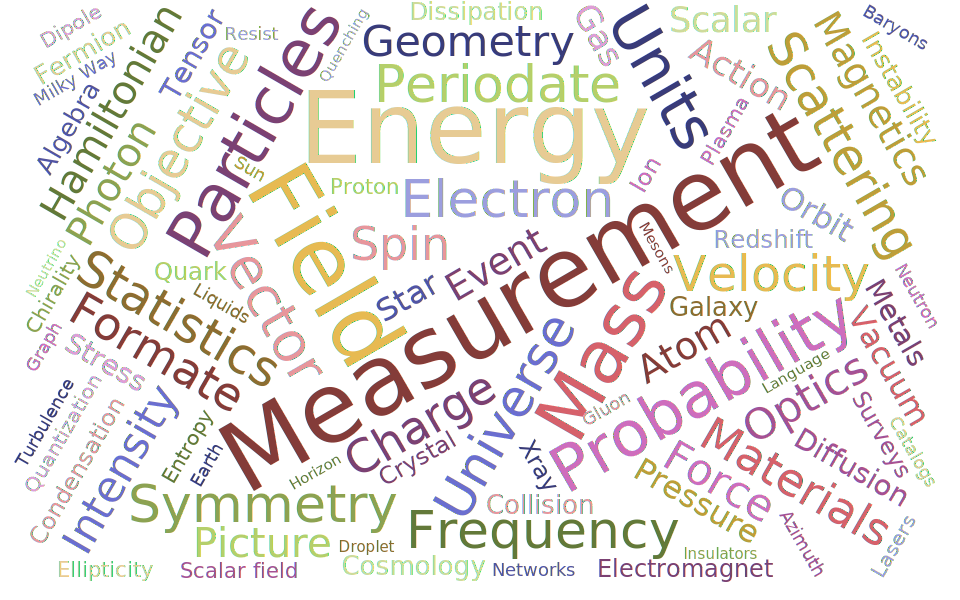
\includegraphics[width=\textwidth]{../img/tagCloud.pdf}}
  \caption{The most common concepts in the corpus, with size representing frequency.}
  \label{fig:tags}
\end{figure}

\baselineskip=16pt
\parindent=15pt
\parskip=5pt

\begin{abstract}
In this paper we derive an {\em effective ontology} by estimating  the {\em interaction strength} between scientific concepts from their use in the scientific literature. This is done by applying the principle of maximum entropy to map the system onto an {\em Ising model} --- a well known model of ferromagnetism in statistical physics --- that is then solved with a pseudolikelihood maximization approach.
The network thus formed is partitioned with {\em community detection} to find clusters of concepts related to each other.
\end{abstract}
\newpage
\section*{Acknowledgments}
I would like to express my gratitude to Professor Paolo De Los Rios for proposing and supervising this project --- his guidance has been very valuable. I would also like to thank Duccio Malinverni  for his support, advice, and continuous availability throughout the project,
Finally, I would like to express my appreciation for the networking and clustering techniques suggested by Andrea Martini.
{\hypersetup{linkcolor=black}
\small
\tableofcontents
}
\newpage
\section{Introduction}

Scientific papers (available e.g. from arXiv\footnote{\url{http://arxiv.org/}}) can be classified according to the concepts they contain, and studying their relationships can lead to a useful and automatic hierarchical grouping of papers.
An issue that has received less attention is the way concepts are related with each other.
Intuitively, concepts that often appear together in papers are related to each other, but of course the precise intensity of this connection is not known.
Moreover, the ensemble of all these connections defines a network, whose structure is presently not known.
The relation between concepts has been already explored in other domains. However, connections are typically defined a priori according to their semantic definitions, and are just binary --- namely, there is or there isn't a connection. This relation network is what we call an {\em ontology}~\cite{guarino1998}.

We propose to analyze the corpus of 54198 scientific articles published in arXiv during 2013 in physics (see table~\ref{tab:cats}).
From these papers {\em concepts} have been extracted and have passed a procedure of collaborative validation from physicists using ScienceWise\footnote{\url{http://sciencewise.info/}}.
The number of papers with at least one article is 52979.
We do not consider directly the correlation between concepts --- it can be trivially calculated --  but rather to try find insights about the causal ties.
This is achieved by adapting a method of interaction--strength inference that has been recently introduced by statistical physicists and that is rapidly gaining ground in different domains such as biology, computer science, social sciences, neuroscience, etc.

In order to do so we derive an {\em Ising model} for the concepts in the articles, and solve an optimization problem to deduce the parameters that best determine the interaction between concepts.
To continue the analogy with statistical physics, we want to estimate the force of attraction or repulsion between concepts.
This has been done already by Floretta~\cite{flo2014} using mean-field inversion.
We propose a method that uses {\em pseudolikelihood maximization} instead.

We then used the interactions to form a network, where each node represents a concept.
Techniques to subdivide network into highly connected groups of nodes have been developed in graph theory and complex networks~\cite{newman2004}.
By exploiting these techniques we attempt to construct a division of the network based on {\em community detection}.

\begin{table}[h]
  \begin{center}
    \begin{tabular}{lrr}
    \hline
    Abbreviation & Papers & Percentage [\%] \\
    \hline
    astro-ph & 12475 & 23.4 \\
    cond-mat & 12749 & 24.0\\
    gr-qc & 2274 & 4.3\\
    hep-ex & 943 & 1.8\\
    hep-lat & 726 & 1.4\\
    hep-ph & 4630 & 8.7\\
    hep-th & 3367 & 6.3\\
    math-ph & 1771 & 3.3\\
    nlin & 880 & 1.7 \\
    nucl-ex & 529 & 1.0\\
    nucl-th & 1294 & 2.4\\
    physics & 7476 & 14.1\\
    quant-ph & 4044 & 7.6\\
    \hline
    Total & 54198 & 100.0 \\
    \hline
    \end{tabular}
  \caption{\label{tab:cats} Composition of our corpus: number and percentage of articles in each arXiv category.}
  \end{center}
\end{table} 
\section{The Ising Model}
\subsection{Definitions}
In order to formulate the problem we have adapted a method to detect protein folding from sequence alignments --- in particular we follow very closely the derivation by Ekeberg~\cite{eke2012}. 

The presence of a concept in an article can be viewed as a binary variable --- it is present or not.
In analogy to the study of ferromagnetism in statistical physics, we represent this as a spin state, that can assume the value 0 or 1.\footnote{This choice is completely arbitrary, as one can label the spins with whichever pair of values one chooses, and the equations remain the same. For example, one can prove that any result is invariant under the transformation $\bf s \mapsto \alpha \bf s + \beta,~\alpha,\beta \in \mathbb{R}$, with appropriate modifications of the field and coupling parameters.}
Using $n$ for the number of concepts and $N$ for the number of articles, we can represent an article by a set of $n$ spins: $\bf{s}=(s_1,s_2,\dots,s_n)$ where $s_i = \{0,1\}\,~\forall\,i=1,\dots,n$.\footnote{Unless stated otherwise, the indices $i,j,k \in 1,\dots,n$.} Therefore, the entire corpus of articles can be viewed as a $N$-tuple of these sets, represented in matrix form as
\be
s\equiv \{\bf s\}_{a=1}^N \equiv
  \begin{pmatrix}
  s_1^{(1)}  & s_2^{(1)} & \dots  & s_n^{(1)}  \\
  s_1^{(2)}  & s_2^{(2)} & \dots  & s_n^{(2)}  \\
  \vdots  & \vdots & \ddots  & \vdots \\
  s_1^{(N)}  & s_2^{(N)} & \dots  & s_n^{(N)}  \\
  \end{pmatrix}
  \label{eq:smatrix}
\ee
\begin{figure}
  \centerline{\includegraphics[width=0.3\textwidth]{../img/dots.png}}
  \caption{\em Spin matrix: full dots mark concepts that are present in an article.}
  \label{fig:dots}
\end{figure}

A visual example is presented in fig.~\ref{fig:dots}.
We define the individual and pairwise {\em frequencies} along the columns to be
\begin{subequations}
  \begin{align}
    f_i &\equiv \langle s_i \rangle = \frac{1}{N} \sum_{a=1}^N s_i^{(a)} \\
    f_{ij} &\equiv \langle s_i s_j \rangle = \frac{1}{N} \sum_{a=1}^N s_i^{(a)}s_j^{(a)}
  \end{align}
  \label{eq:fdef}
\end{subequations}
The $f_{i}$ represent the probability the $i$-th concept is present. 
Instead the pairwise frequencies $f_{ij}$ represent the the $i$-th and $j$-th appear together in an article.
The total number of concepts we work with is 13174; a visualization of the most common concepts in the entire corpus is presented in fig.~\ref{fig:tags}.

\subsection{Principle of Maximum Entropy}
We are interested in deriving a probabilistic model $\P(\bf s)$ of the concept interactions that is compatible with the empirical observations, but at the same time can describe these interactions in the most general way.
This is achieved by applying the {\em principle of maximum entropy}, which states that the probability distribution that represents the empirical observations must  maximize the entropy~\cite{jaynes1957}.

Although it may seem odd to apply a principle of statistical mechanics to a situation with no physical basis, it can be interpreted from an information theory point of view, expressing the epistemological modesty of our view of the system.
In fact this principle is compelling because choosing a distribution that maximizes entropy suggests the state of least information.
A state with lower entropy would imply that there is unknown information; therefore the states with maximum entropy express the situation of ``most ignorance''.

Explicitly, the {\em entropy} of the system is defined as
\be
  S \equiv - \sum_{\{s_k= 0,1\}} \P(\bf s) \ln \P(\bf s)
  \label{eq:sdef}
\ee
where $\sum_{\{s_k= 0,1\}} \equiv \sum_{\bf s}$ indicates the sum over all possible configurations of $\bf s$.

The distribution $\P(\bf s)$ must satisfy the constraints of being with the experimental observations $f_i$ and $f_{ij}$. This condition is expressed as
\begin{subequations}
  \begin{align}
    &\sum_{\bf s} s_i \P(\bf s) = f_i \\
    &\sum_{\bf s} s_i s_j \P(\bf s) = f_{ij} 
  \end{align}
  \label{eq:pconsistency}
\end{subequations}
and $\P(\bf s)$ is normalized
\be
  \sum_{\bf s} \P(\bf s) = 1
  \label{eq:pnorm}
\ee

The maximization of the entropy in \eq{eq:sdef} under the constraints in \eq{eq:pconsistency} and \eq{eq:pnorm} is achieved with the Lagrange multipliers, ie. solving
\begin{align}
  \frac{\delta}{\delta \P(\bf s)}\left [ -\sum_{\bf s} \P(\bf s) \ln \P(\bf s)
    + \lambda_0\( \sum_{\bf s} \P(\bf s)-1\) 
    + \sum_i\lambda_i \( \sum_{\bf s} s_i \P(\bf s) - f_i \) \right. \nonumber\\
    \left. + \sum_{i,j}\mu_{ij} \( \sum_{\bf s} s_i s_j \P(\bf s) - f_{ij} \) \right ]= 0 \nonumber
  \label{eq:multipliers}
\end{align}
After a straightforward derivation, and after reabsorbing the constants we find
\be
  \ln \P(\bf s) = \lambda_0 + \sum_i \lambda_i s_i + \sum_{i,j} \mu_{ij} s_i s_j \nonumber
\ee
In a notation that is more customary with Ising models, this becomes
\be
  \P(\bf s) = \frac{1}\part\exp{{\ham(\bf s)}}
  \label{eq:pdist}
\ee
where
\be
  \ham(\bf s) = \sum_i h_i s_i + \sum_{i}\sum_{j>i} J_{ij} s_i s_j 
\ee
and the {\em partition function} $\part$ derives directly from \eq{eq:pnorm}
\be
  {\cal Z} = \sum_{\bf s} \exp{\ham(\bf s)}
  \label{eq:partdef}
\ee
The {\em field} $\bf h = \{h_i\}$ and {\em coupling} $\bf J = \{J_{ij}\}$ are the parameters that determine the distribution function. 
As mentioned before, they must satisfy \eq{eq:pconsistency}.
Just as a matter of notation, since $J_{ij} = J_{ji}$ (the pairwise interactions are not directional) we can avoid double-counting of the pairwise interactions by summing over $\sum_i\sum_{j>i}$.

\paragraph{A note on the Intractability of $\part$} Considering \eq{eq:partdef} we notice that even if the $\{\bf  h,\bf J\}$ are known, the computational time required to evaluate $\part$  becomes enormous very rapidly ---its complexity is around  $\order(n^2 2^n)$. 
For our case where $n \approx 10^4$ an exhaustive evaluation remains completely outside consideration from a practical point of view.
We therefore will have to resort to methods that avoid this.
\section{Method Development}
\subsection{Maximum Likelihood Estimation}
Given a set $\{\bf s\}_{a=1}^N$ of  observations we want to determine the parameters $\{\bf  h,\bf J\}$.
The standard statistical approach is to maximize the {\em likelihood},
\be
  {\cal L}(\bf h,\bf J) = \prod_{a=1}^N \P(\bf s^{(a)})
  \label{eq:likedef}
\ee
Indeed the likelihood of the set of parameters  $\{\bf  h,\bf J\}$ is equal to the probability of measuring the observed outcomes given that set of parameters.
A maximum likelihood estimator coincides with the most probable Bayesian estimator, assuming the set of observations is independent, i.e. there is no correlation between the different $\bf s^{(a)}$.
For practical reasons it is much more convenient to minimize the average {\em negative log-likelihood}~\cite{eke2012}
\be
  \ell(\bf h,\bf J) \equiv -\frac{1}{N}\sum_{a=1}^N \ln \P(\bf s^{(a)})
  \label{eq:nlldef}
\ee
Therefore the estimators can be obtained by minimizing \eq{eq:nlldef}, i.e.
\be
  \{\bf h^{\rm MLE}, \bf J^{\rm MLE}\} = \arg\min \ell(\bf h,\bf J)
\ee
Attempts to apply this in our case --- plugging \eq{eq:partdef} into \eq{eq:nlldef} and then deriving $\ell$ to find the minima --- are illustrated in literature~\cite{eke2012}.
Unfortunately this yields a result that  is explicitly dependent of the partition function.
As illustrated previously, in order to have an estimator it is necessary to get rid of explicit dependencies in $\part$.

\subsection{Pseudolikelihood Approximation}
A method to avoid full-space normalization is to use the {\em pseudolikelihood} as an approximation of the likelihood that has spatial dependencies~\cite{oxfordstat}\cite{eke2012}.
Using the definition of {\em conditional probability}
\be 
  \P(A|B)=\frac{\P( A \bigcap B) }{\P(B)}
  \nonumber
\ee
we can derive the conditional probability of having $s_k$ given all the other spins.
By denoting $\sminusk = (s_1,\dots,s_{k-1},s_{k+1},\dots,s_n)$ we have
\be
  \P(s_k | \sminusk) = \frac{\P(s_k,  \sminusk)}{\P( \sminusk)}
  = \frac{\P(\bf s)}{\P(s_k=0,  \sminusk) +\P(s_k=1, \sminusk)}
\ee
We can insert \eq{eq:pdist} and cancel all terms that do not contain $s_k$
\be
  \P(s_k | \sminusk) = \frac{\exp \( h_k s_k + \sum_{j \neq k} J_{jk} s_j s_k\) }{1+\exp \( h_k + \sum_{j \neq k} J_{jk} s_j\) }
  \label{eq:condprob}
\ee
We notice  at this point that the the dependency in $\part$ has been eliminated. We use the denominator in \eq{eq:condprob} as an approximation for the partition function for the site $k$.
By summing over $k$ and our set of articles we can define {\em negative pseudo-log-likelihood} in a form that is similar to \eq{eq:nlldef}
\be
  \hat{\ell}(\bf h,\bf J) = -\frac{1}{N}\sum_{a=1}^N \sum_k \ln \P(s_k^{(a)} | \sminusk^{(a)})
  \label{eq:nplldef}
\ee
The estimators of ${\bf h,\bf J}$ are therefore obtained by minimizing $\hat{\ell}$
\be
  \{\bf h^{\rm PLM}, \bf J^{\rm PLM}\} = \arg\min \hat{\ell}(\bf h,\bf J)
  \label{eq:npllest}
\ee
It is important to note that in general the estimators $\{\bf h^{\rm PLM}, \bf J^{\rm PLM}\}$ which maximize the pseudolikelihood do {\em not} maximize the likelihood, i.e. satisfy \eq{eq:nlldef}.
It is however considered a valid approximation that often leads to meaningful results~\cite{oxfordstat}.

\subsection{Regularization}
What we did not mention about \eq{eq:npllest} is that there may be multiple solutions, we prefer, however, the ones with most terms at zero, since they can describe the system with the minimal amount of interactions.
Additionally it helps the convergence of the numerical optimization.
As a matter of fact, $\hat{\ell}$ is convex --- therefore a solution is always expected, but is extremely very flat around zero.
As has previously been shown by Ekeberg~\cite{eke2012}, the standard way of doing this is introducing a {\em penalty function} $R$, so that \eq{eq:npllest} becomes
\be
  \{\bf h^{\rm PLM}, \bf J^{\rm PLM}\} = \arg\min \( \hat{\ell}(\bf h,\bf J) + R(\bf h,\bf J) \)
  \label{eq:npllestreg}
\ee
This procedure is called {\em regularization}~\cite{oxfordstat}, and in particular we choose to regularize using the $L^2$ norm, which is a convenient choice because it maintains the function to minimize differentiable.
 Using arbitrary positive constants $\lambda_h$ and $\lambda_J$, our penalty function becomes
\be
  R(\bf h,\bf J) = \lambda_h \sum_{i} h_i^2 + \lambda_J \sum_i\sum_{j < i} J_{ij}^2
  \label{eq:l2norm}
\ee
We see that $R$ pushes collectively the parameters towards zero.
In fact to minimize $R$ the Euclidean norms of $\bf h$ and $\bf J$ should separately be the smallest possible.
The $\lambda$ constants are chosen by striking a compromise between accurately fitting the data and maintaining small parameters.
\subsection{Gradient of the Objective Function}
It is now formulate the problem as a function optimization.
Using \eq{eq:condprob} and \eq{eq:nplldef}, we can find an explicit formulation for $\hat{\ell}$
\be
  \hat{\ell} (\bf h,\bf J)= -\frac{1}{N}\sum_{a=1}^N\sum_k \vast[ h_k s_k^{(a)} + \sum_{j \neq k}J_{jk} s_j^{(a)} s_k^{(a)} - \ln\vast( 1+\exp \(  h_k + \sum_{j \neq k} J_{jk} s_j^{(a)}\) \vast) \vast]
  \nonumber
\ee
We now define $F(\bf h,\bf J) \equiv \hat{\ell}(\bf h,\bf J) + R(\bf h,\bf J)$ as the {\em objective function}. 
Introducing the frequencies of \eq{eq:fdef}  we get
\be
  F = \sum_k   \vast[  - f_k h_k - \sum_{j \neq k} - f_{jk} J_{jk} + \frac{1}{N}\sum_{a=1}^N \ln\vast( 1+\exp\( h_k + \sum_{j \neq k} J_{jk} s_j^{(a)}\) \vast) \vast] + R
  \label{eq:objfuncexpl}
\ee

Since $F$ is well-behaved the minimum of \eq{eq:npllestreg} can be found by deriving $F$ along our parameters, i.e. when $\grad_{\{\bf h,\bf J\}} F(\bf h,\bf J) = \bf 0$.
Using \eq{eq:l2norm} and \eq{eq:objfuncexpl} we obtain
\begin{subequations}
  \begin{align}
    &\partial_{h_i}F = -f_i + 2\lambda_h h_i +\frac{1}{N} \sum_{a=1}^N\frac{\exp\( {h_i} + \sum_{k \neq i}J_{ik}s_k^{(a)} \) }{ 1+\exp\( {h_i} + \sum_{k \neq i}J_{ik}s_k^{(a)}\) }  = 0 \\
   & \partial_{J_{ij}}F = -f_{ij} + 2\lambda_J J_{ij} +\frac{1}{N} \sum_{a=1}^N s_j^{(a)} \frac{\exp\( h_i + \sum_{k \neq i}J_{ik} s_k^{(a)}\) }{ 1+\exp\( h_i + \sum_{k \neq i} J_{ik} s_k^{(a)}\) }  = 0
  \end{align}
\label{eq:derivatives}
\end{subequations}
This set of equations is coupled, non-linear and not solvable analytically. 
We have however reduced the search for the field and coupling parameters to an optimization problem, that can be solved  with numerical methods.

\subsection{Notation with Triangular Matrices}
To simplify the notation, let us introduce some new variables.
We combine the field and couplings in a {\em lower triangular matrix}, so that the field is in on the diagonal elements. Similarly we generalize $f_{ij}$ to contain the individual frequencies on the diagonal, and $\lambda_{ij}$. This is equivalent to
\be
x_{ij} \equiv 
  \left\{
    \begin{array}{ll}
      J_{ij}  & \mbox{if } i > j \\		
      h_i & \mbox{if } i = j \\
      0 & \mbox{if } i < j
  \end{array}
\right. ,\;
f_{ij} \equiv 
  \left\{
    \begin{array}{ll}
      f_{ij}  & \mbox{if } i > j \\		
      f_i & \mbox{if } i = j \\
      0 & \mbox{if } i < j
  \end{array}
\right. ,\;
\lambda_{ij} \equiv 
  \left\{
    \begin{array}{ll}
      \lambda_h  & \mbox{if } i = j \\		
      \lambda_J & \mbox{if } i \neq j 
  \end{array}
\right.
\ee
The objective function and its derivatives can be rewritten in a more compact form by defining
\be
  \xi_i^{(a)}\equiv\exp\( x_{ii} + 2\sum_{k < i} x_{ik} s_k^{(a)}\)
\ee
Finally we have
\begin{subequations}
  \begin{empheq}[box=\fbox]{align}
  &F = \sum_i \( - \sum_{j \leq i}f_{ij}x_{ij} + \sum_{j \leq i}\lambda_{ij} x_{ij}^2 + \frac{1}{N}\sum_{a=1}^N \ln\( 1+\xi_i^{(a)} \) \) \label{eq:funcgrad:func}\\
  &(\grad F)_{ij} = -f_{ij} + 2\lambda_{ij} x_{ij} +\frac{1}{N} \sum_{a=1}^N \left \{s_j^{(a)}\right \}_{i \neq j} \frac{\xi_i^{(a)} }{ 1+\xi_i^{(a)} }  \label{eq:funcgrad:grad}
  \end{empheq}
  \label{eq:funcgrad}
\end{subequations}
where we write $\{s\}_{i \neq j} \equiv  \delta_{ij} + (1-\delta_{ij})s$ using the Kronecker delta $\delta_{ij}$.

\section{Algorithm}
\subsection{Overview}
A {\em steepest descent} algorithm finds the minimum of a function given its gradient, which is exactly what we have in this situation, see \eq{eq:funcgrad}. 
This technique translates $x$ of an $n$-dimensional vector along the negative gradient, i.e. where the function descends the fastest.
The library we chose\footnote{ ALGLIB, see \url{www.alglib.net}} uses a  improved method, called L-BFGS, that stands for {\em Limited-memory  Broyden--Fletcher--Goldfarb--Shanno}.
This algorithm keeps a history of a certain number of the previous updates to approximate the inverse Hessian.
It can therefore build a quadratic model and get a better idea of what the function looks like, hopefully converging faster towards the minimum.
\subsection{Description}
\begin{algorithm}
\setstretch{1.25}
\DontPrintSemicolon
\KwData{Spin matrix $s$}
\KwResult{Parameter matrix $x$}
\BlankLine
\Begin{
  compute frequency matrix $f$\;
  $x \asg {\bf 0}$\;
  \While{$\neg$haltingCondition}{\label{alg:main:starteval}
    $F \asg 0$, $\grad F \asg \bf{0}$\;
    \For{$ i=1,\dots,n$}{
      $\Sigma \asg 0$\tcp*[r]{Stores the log sum}
      \For{$ a=1,\dots,N$}{
        $\theta \asg x_{ii}$\tcp*[r]{Stores the exp argument}
        \For{$j : s_{ij}^{(a)} = 1$}{
          $\theta \asg \theta + x_{ij}$\;
        }
        $\xi \asg \exp(\theta)$ \label{alg:main:expon}\tcp*[r]{Different name for clarity}
        $\Sigma \asg \Sigma + \log(1+\xi)$\;\label{alg:main:logsum}
        $(\grad F)_{ii} \asg (\grad F)_{ii} + \xi/(1+\xi)$\;\label{alg:main:gradpartdiag}
        \For{$ j : s_{ij}^{(a)} = 1$}{
          $(\grad F)_{ij} \asg (\grad F)_{ij} +  \xi/(1+\xi)$\;\label{alg:main:gradpartsubdiag}
        }
      }
      $F \asg F + \Sigma/N - f_{ii} x_{ii} + \lambda_h x_{ii}^2$\;\label{alg:main:fdiagreduce}
      $(\grad F)_{ii} \asg (\grad F)_{ii}/N - f_{ii} + 2\lambda_h x_{ii}$\;
      \For{$j < i$}{
        $F \asg F - 2f_{ij} x_{ij} + \lambda_J x_{ij}^2$\;
       $(\grad F)_{ij} \asg (\grad F)_{ij}/N - f_{ij} + 2\lambda_J x_{ij}$\;\label{alg:main:endeval}
      }
    }
    \tcp{Values of previous iterations  are implicitly used for these steps}
    $x \leftarrow {\rm LBFGS}step(F,\grad F,x)$\;\label{alg:main:lbfgs}
    update $haltingCondition$\;\label{alg:main:updatehalt}
  }
}
\caption{Calculation of the objective function and its gradient for the optimization routine.}
\label{alg:main}
\end{algorithm}
We now present a more detailed description of the numerical optimization (see algorithm~\ref{alg:main}).
For the initialization step the frequency matrix is initially calculated using eq.~\ref{eq:fdef}.
The objective function $F$ and its gradient $\grad F$ are calculated in lines~\ref{alg:main:starteval}-\ref{alg:main:endeval}. This is achieved by iterating over the indexes $i,a$ and calculating the exponential $\xi$ that is found in \eq{eq:funcgrad}.
Notice that for clarity we store the exponential and its argument in separate variables.
This is however unnecessary and we can very well store this in the same variable, i.e. line~\ref{alg:main:expon} becomes $ \xi \leftarrow \exp(\xi)$.

We can now keep the sum of the logarithmic terms for $F$ in a temporary variable (see line~\ref{alg:main:logsum}) $\Sigma$ and update the gradient terms $(\grad F)_{ij}$ in lines~\ref{alg:main:gradpartdiag}-\ref{alg:main:gradpartsubdiag}.
The sum $\Sigma$ is then added to $F$, along with the other  terms polynomial in $x$. Similarly, the partial sum in $(\grad F)_{ij}$ is divided by $N$ and the rest of the terms are added (lines~\ref{alg:main:fdiagreduce}-\ref{alg:main:endeval}).

We then use $F$ and $\grad F$ to update $x$ using the L-BFGS method (line~\ref{alg:main:lbfgs}). 
The operations on lines~\ref{alg:main:lbfgs}-\ref{alg:main:updatehalt} actually use $F$, $\grad F$ and $x$ of previous iterations.
We mentioned before that the optimization algorithm uses the previous values to tune the next translation step.
But in order to compute the stopping conditions we must also store the values of the previous iteration.
For example as a halting condition we choose
\be
  | F_{m+1} - F_m | \leq \epsilon_F\max(|F_{m+1}|,|F_m|,1)
  \label{eq:halting}
\ee
where $F_m$ denotes the value of $F$ at the $m^{\rm th}$ step of the routine.
The constant $\epsilon_F$ is chosen by the user and  determines how close we want to be to the actual minimum.

For {\em each} function and gradient evaluation, the time complexity is $\order(n^2 N)$. Since the dimensionality of our problem is quite high, the number of operations per iterations is quite important --- probably at least $10^{12}$. This makes the evaluation of the function and gradient the most time--consuming part compared to the optimization step of the algorithm.

To read how the algorithm was implemented, see appendix~\ref{section:tech}.

\section{Verification}
\subsection{Random Matrices}
\begin{figure}
  \centerline
  {
    \includegraphics[width=0.9\textwidth]{../img/distribution_random.pdf}
  }
  \caption{Comparison of the probability density function $f$ for different values of $\lambda$ for random matrix of dimensions $n=200$, $N=25000$. The continuous lines correspond to a Gaussian fit.}
  \label{fig:randdist}
\end{figure}
It is not simple to verify the validity of the algorithm, as the results are not something directly measurable. 
However, one ne way of verifying the algorithm is to use a {\em random matrix} for the spins, formed by  independent random variables with a uniform distribution.
By definition the system should have no correlations, because the spins are independent random variables.
The corresponding Ising model will have a Gaussian distribution depending on the renormalization constant $\lambda$.\footnote{From now on we set $\lambda_h = \lambda_J \equiv \lambda$. }
Introducing the penalty function \eq{eq:l2norm} in the negative log-likelihood \eq{eq:nlldef}
\be
  \ell^\prime(x) = -\frac{1}{N}\sum_{a=1}^N \( \ln \P(\bf s^{(a)}) - \lambda \| x \|^2 \) \nonumber
\ee
where  $\| x \|^2 \equiv \Tr(x^\intercal x)$ denotes the Frobenius matrix norm.
We return to the expression of the likelihood, which has the form
\be
  {\cal L}^\prime(x) = \underbrace{{\cal L}(x)}_{\rm constant} \e^{ - N \lambda \| x \|^2 }
\ee
since the distribution of $\bf{s}^{(a)}$ is uniform and independent of the index $a$. 
From this form we deduce that the parameter distribution centered on zero, with standard deviation $\sigma = 1/\sqrt{2 N \lambda}$. 
Therefore in Bayesian statistics the regularization term corresponds to a {\em prior}, that is the expected distribution that the parameters should have before considering the empirical data~\cite{oxfordstat}.

This prediction is indeed confirmed by what we qualitatively measure by binning the different parameters $x_\alpha$\footnote{The index $\alpha$ is used to indicate a generic index pair $(i,j)$.} by their value and looking at their distribution (see fig.~\ref{fig:randdist}). 
The parameters are spread around zero with a variance that is inversely proportional to $\lambda$. 
From now on we shall choose to take $\lambda = 0.01$. 
This value is what is usually found in literature for inferences in protein sequences, but does not guarantee good results in this case.
A full study of the prior parameter has not been attempted because of time constraints and the time complexity of our implementation.
\subsection{Comparison with J Domain Results}
The algorithm proposed was tested on results derived from {\em J domain} protein sequencings provided by Duccio Malinverni.
These results were obtained using an asymmetric version of a pseudolikelihood inference on a Potts model, so the initial sequences had to binarized accordingly.
Nonetheless, our results have a similar distribution and are strongly correlated (see fig.~\ref{fig:jdmdist}).
The absolute value is taken as the results we compare with are all positive because they are under a different gauge.
Finally, one can qualitatively compare the results by looking at the patterns in the couplings, as shown in fig.~\ref{fig:jdmcouplings}. 
The signatures are convincingly similar.
\begin{figure}
  \centerline{
    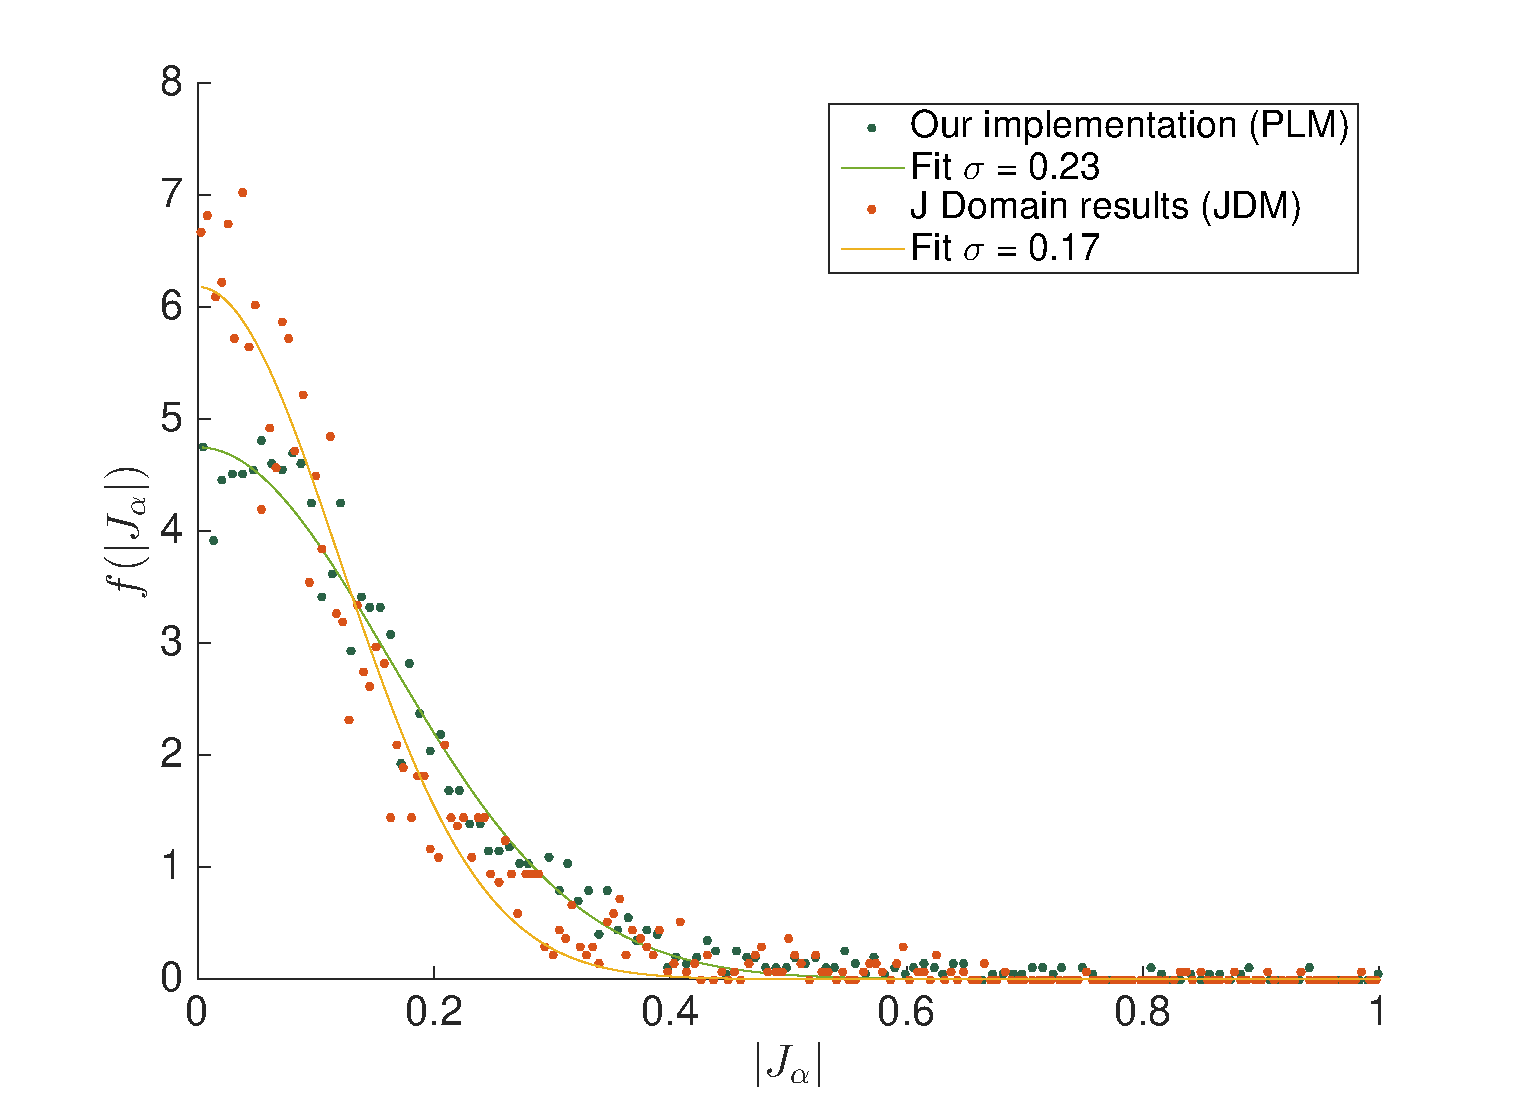
\includegraphics[height=6cm,width=\textwidth,keepaspectratio]{../img/distribution_jdm.pdf}
    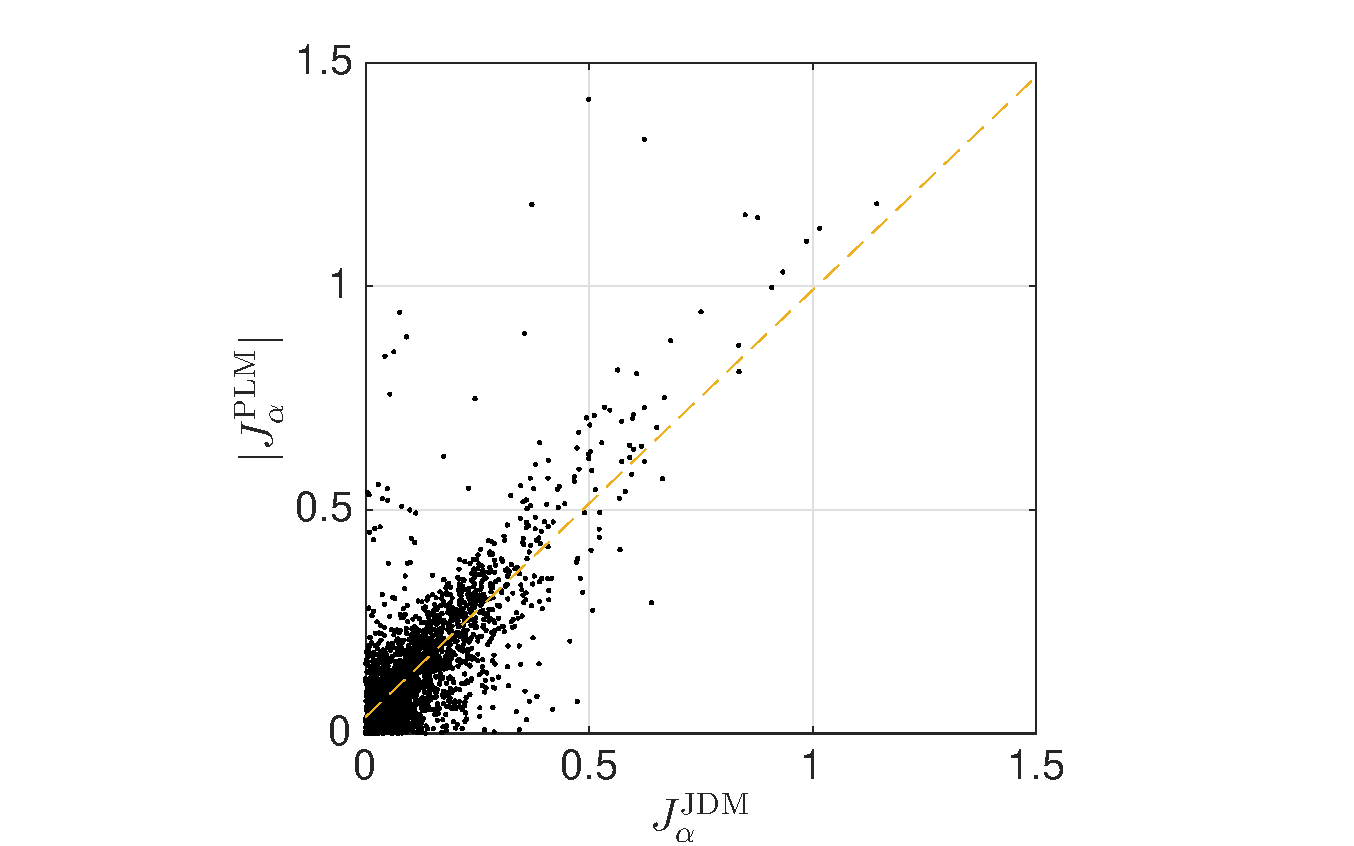
\includegraphics[height=6cm,width=\textwidth,keepaspectratio]{../img/correlations_jdm.pdf}
    }
  \caption{{\em Left}: comparison of the couplings distribution for the two methods. {\em Right}: correlations between the couplings of the two methods. The yellow line represents a linear fit.}
  \label{fig:jdmdist}
\end{figure}
\begin{figure}
  \centerline{
    \includegraphics[width=0.8\textwidth]{../img/couplings_jdm.png}
  }
  \caption{Visualization of the couplings matrix.}
  \label{fig:jdmcouplings}
\end{figure}

\section{Community Detection}
\subsection{Graph Construction}
We have the couplings describing the interaction between all concepts. 
The goal now is to bunch them together to find sets of concepts that are tighly connected internally.
There is a great abundance of clustering algorithms available~\cite{jain1999}, but it is difficult to define an appropriate metric (or pseudometric) that defines a distance between concepts.
We resort to mapping the coupling matrix to an {\em undirected graph} or network, where each concept is identified with a vertex.
Attemping to incorporate the values of the couplings in edge weights is not a trivial problem.
Couplings can assume all values in $\mathbb R$, while weights have to be stricty positive, with larger weights corresponding to weaker interactions, the opposite of couplings.
We therefore decided to crudely binarize the couplings according to a {\em threshold value} $J_\bot$, such that all couplings under this value were set to zero (corresponding to breaking the graph edge corresponding to the coupling) and adding an edge for each coupling larger than $J_\bot$. 

Once our graph has been defined we can attempt to find a {\em community structure}, by partitioning the network into {\em communities} that contain highly interconnected nodes, while nodes of different communities are only sparsely connected~\cite{newman2004}.
We focus on approaches based on the optimization of a quantity called the {\em modularity}, which roughly measures the density of edges inside communities to edges outside communities.

For a network partition into $m$ different communities, we define the $m \times m$ symmetric matrix $e$ such that $e_{vw}$ is the fraction of all edges in the network that link vertices in community $v$ to vertices in community $w$. 
The sum of the diagonal components of $e$ indicates the fraction of edges that fall into the community partition.
This must however weighed against a network with the same partition with random edges~\cite{newman2004}.
In this notation we define the modularity as
\be
  Q = \Tr(e) - |\bf{a}|^2 
\ee
where we write the sum of $e$ over an index as $a_v = \sum_{w} e_{vw}$.
Therefore the modularity measures the fraction of edges falling into the given communities compared with the expected value if the edges were distributed at random.
If the number of community edges is equivalent to random connections, we obtain $Q = 0$. A  value of $Q$ approaching 1 indicates a partition highlighting a strong community structure.
Exact maximization of the modularity is believed to be an NP-complete problem, but fortunately several heuristic algorithms have been proposed.
We choose to use the {\em Louvain Method}~\cite{blondel2008}, known for empirically running in linearithmic time.
\subsection{Full Dataset}
\begin{figure}
  \centerline{
    \includegraphics[height=6cm,width=0.6\textwidth,keepaspectratio]{../img/distribution_comparison.pdf}
    \includegraphics[height=6cm,width=0.5\textwidth,keepaspectratio]{../img/tscan.pdf}
  }
  \caption{Distribution of couplings compared to the null model ({\em left}) and fraction of points over the quartile in function of $t_\gamma$ ({\em right}).}
  \label{fig:distcomp}
\end{figure}
The distribution of the couplings obtained with the full dataset are presented in fig~\ref{fig:distcomp}. The results are compared with the distribution for a random matrix that the same individual concept frequencies.
This allows us to use the uncorrelated couplings as a {\em null model}.
We then introduce the quantity $t_\gamma$ that is the value of $J$ corresponding to $\gamma$-quantile of the null model.
Thus, by choosing $t_\gamma$ correctly, we effectively select the part of couplings we consider significant.

Using the whole dataset does not yield a significant community structure.
This may be caused by many factors, including a too stringent prior, or a large difference in frequencies. 
In fact the statistic may not be sufficient to reconstruct accurately the interaction of concepts that appear very rarely in the dataset.

\subsection{Subset of Most Frequent Concepts}
\begin{figure}
  \centerline{
    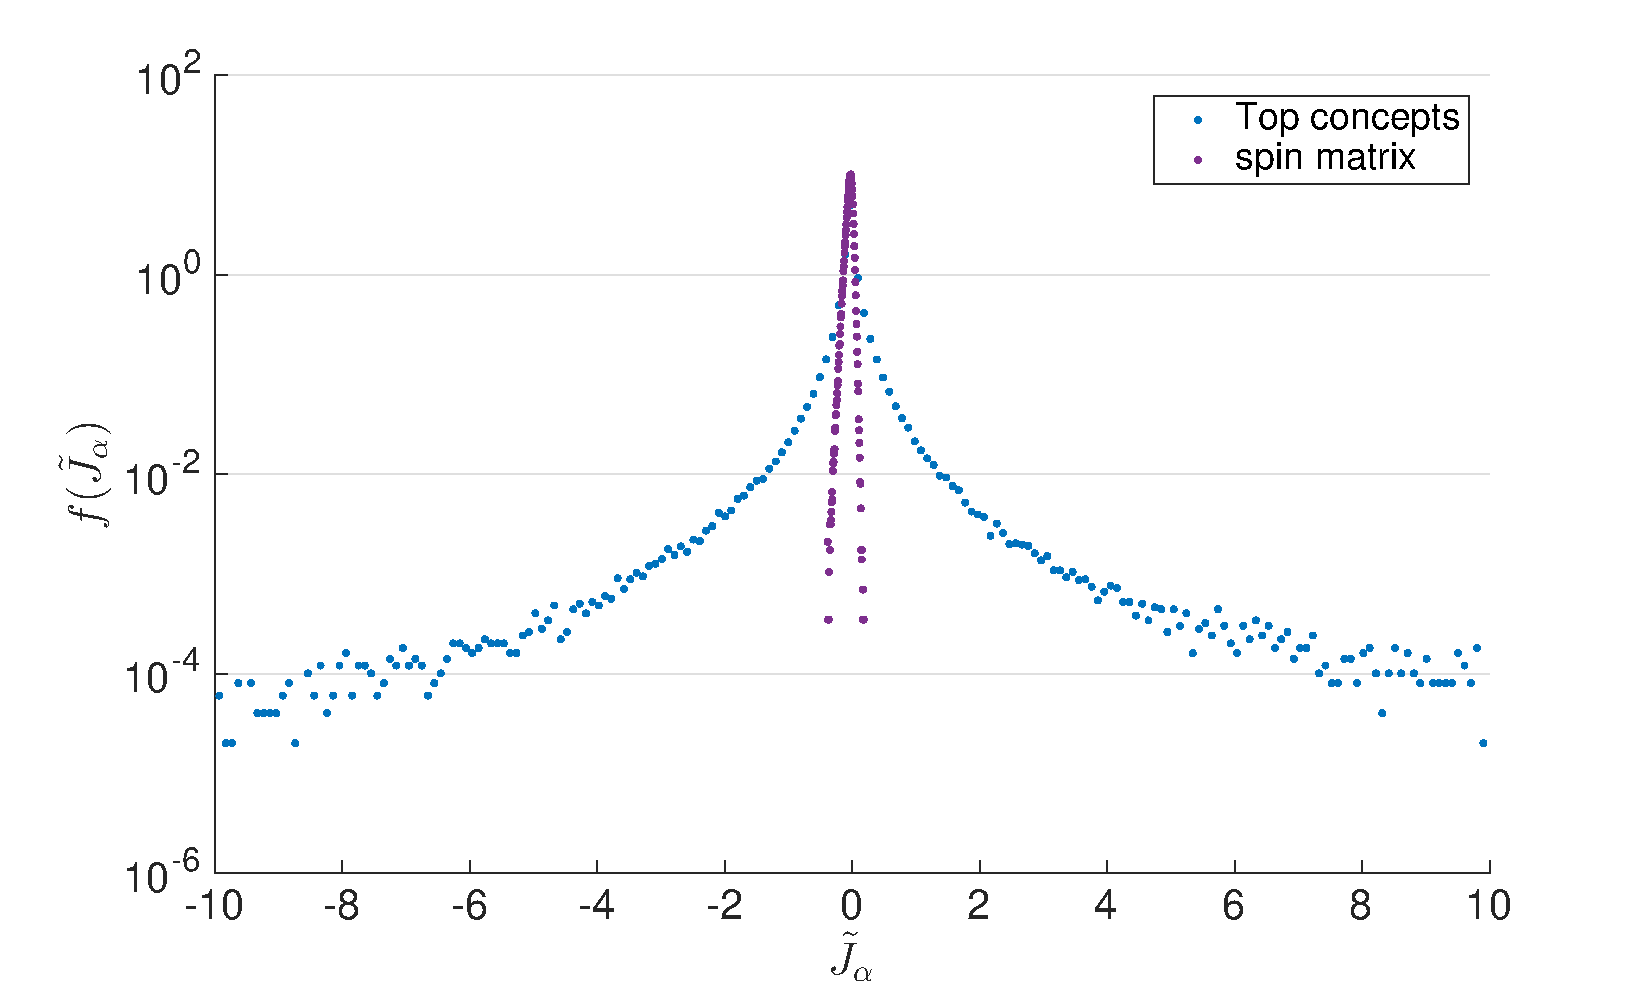
\includegraphics[height=6cm,width=1\textwidth,keepaspectratio]{../img/distribution_comparison_top.pdf}
    \includegraphics[height=6cm,width=1\textwidth,keepaspectratio]{../img/comparison_top_total.pdf}
  }
  \caption{Distribution of couplings compared to the null model ({\em left}) and  distribution of the concepts by category for the full dataset and the subset ({\em right}).}
  \label{fig:topc}
\end{figure}

We restrict our focus to the first thousand most frequent concepts using a lower regularization factor of $\lambda = 0.001$.
In order to compensate for strong frequency disparities, we introduce the {\em average product correction} is
\be
  \tilde{J}_{ij} = J_{ij} - \frac{|J|_{i \bullet } |J|_{\bullet j}}{|J|_{\bullet \bullet }}
\ee 
where $|J|$ denotes the absolute value of each element and $\bullet$ indicates an average over that index. We then proceed in creating a network with the threshold value $J_\bot = 0.14 \approx t_1$.

One can take a look at some of the results in table~\ref{tab:commlist} of appendix~\ref{section:commlist}.
First for each concept we count the frequency in which it appears in articles associated with each arXiv category.
Therefore we say that a concept is associated  with the category in which it appears the most.
In order to maintain an approximately even  distribution (see table~\ref{tab:cats} and fig.~\ref{fig:topc}), we combine smaller arXiv categories in the following groups:  \bf{hep-*} contains `hep-ex', `hep-lat', 'hep-ph', and `hep-th'; \bf{other} contains `gr-qc', `math-ph', `nlin', `nucl-ex', `nucl-ph', `physics' and `quant-ph' . The categories \bf{astro-ph} and \bf{cond-mat} are kept separately since they contain a large portion of the concepts.

We notice that community $\comm_1$ contains the most frequent concepts in the whole dataset (see table~\ref{tab:commprop}).
These concepts are very generic, indeed they seem to be distributed in each of our categories (see fig.~\ref{fig:comm}).
The best results seem to be obtained for $\comm_3$, $\comm_4$ and $\comm_5$.
 Both from a qualitative analysis and looking at their distribution along the categories they clearly contain keywords related to particle physics, astronomy and condensed matter respectively.
A qualitative analysis of $\comm_2$ suggest it is semantically related to cosmology. 
The distribution in fig~\ref{fig:comm} shows that its concepts belong mostly to \bf{hep-*}, \bf{astro-ph} and \bf{other}. 
This is quite possible since the 'gr-qc' category is contained in \bf{other}, and we expect this field is tightly related to high energy physics and astronomy.
\begin{figure}
  \centerline{
   \includegraphics[height=8cm,width=\textwidth,keepaspectratio]{../img/communities_graph.pdf}
   \includegraphics[height=8cm,width=\textwidth,keepaspectratio]{../img/categories_communities.pdf}
  }
  \caption{{\em Left}: visualization of the network, different communities are highlighted with different colors. {\em Right}: distribution within the different communities of the concepts associated with different categories.}
  \label{fig:comm}
\end{figure}
\begin{table}
  \begin{center}
    \begin{tabular}{c|rrrc}
    $\cal C$ & size & $\overline{f}$ &  $\sigma_f$ & main categories\\
    \hline
    1 & 148 & 0.14 & 0.11  & 	other/astro-ph\\
    2 & 153 & 0.024 & 0.019 &  	hep-*/other\\
    3 & 136 & 0.032 & 0.027 & 	hep-*\\
    4 & 235 & 0.026 & 0.022 &	astro-ph \\
    5 & 235 & 0.026 & 0.016 &	cond-mat\\

    \end{tabular}
  \caption{\label{tab:commprop} Summary of the community properties: size, average frequency $\overline{f}$, standard deviation $\sigma_f$ and the main communities detected.}
  \end{center}
\end{table} 

\section{Conclusion}
In this project we have proposed a method to build an effective ontology of concepts out of a corpus of scientific papers and extract subsets of similar concepts.
By applying the principle of maximum entropy we construct an implicit Ising model, for which we want to determine the parameters.
This is achieved using pseudolikelihood maximization to reduce the problem to a function optimization.
An algorithm is then proposed to solve the problem numerically.

As a proof of concepts, we focused on the first thousand most frequent concepts in our dataset, and proceeded to extract a community structure out of the interaction network so as to identify groups of semantically similar concepts.
We then compared our results with the categorizations within arXiv; this has allowed to validate our method by recognizing that the concepts of each community to belong to a specific category.

The current implementation is not fully mature. 
The biggest challenges lie in the interpretation of the couplings and on the construction of the taxonomy.
For practical purposes we built an undirected graph by using a cutoff value. 
We imagine that more refined techniques which retain more coupling intensity information can be developed. 
Finally, a more careful study of the regularization term should be done to establish which regularization norm and which parameter values are optimal.
Moreover, these details can be tailored for specific applications.

{\em Automated ontology learning} is a topic that has been enjoying growing interest in recent years, both in academia and in commercial applications. 
The extraction of a hierarchy or of an underlying structure will allow a new range of algorithms and services based on semantics rather than syntax~\cite{bonino2004}. 

\begin{quote}
{The source code for this project is available at \\
 \url{https://github.com/giacomogiudice/concepts}}
\end{quote}

\bibliographystyle{plain}
\bibliography{references}

\newpage
\appendix
\section{Technical Considerations}
\label{section:tech}
\paragraph{Implementation} As one can see from the source code, our implementation of algorithm~\ref{alg:main} was developed in {\bf C++}, using an object--oriented approach to subdivide the tasks.
A simplified view of the main classes is presented in  fig.~\ref{fig:flow}.
We can follow the arrows and view the flow of information within the class methods.
The data is initially treated by an instance of the {\tt IO} class, is used to start up the {\tt Optimizer} and initialize correctly the {\tt Function}.
There is then a cycle between {\tt Optimizer::run()} and {\tt Function::evaluate()}, that perform the  optimization steps and the function evaluations respectively.
Finally, the data is saved on the disk.
\begin{figure}[h]
  \centerline{\includegraphics[width=9cm]{../img/classes.png}}
  \caption{Flow of calls to the class methods.}
  \label{fig:flow}
\end{figure}


\paragraph{Data Structures} Regarding data structures, the triangular matrices in \eq{eq:funcgrad} are stored as an array, rather than a matrix so as to not waste memory storing the upper diagonal, which is zero.
Therefore one must change indices when accessing memory: this is achieved with the change of indices
\[
  (i,j) \mapsto \alpha = \frac{i (i+1)}{2} + j,\; i \geq j
 \]
 so that $x_\alpha = x_{ij}$.
 
It is worth mentioning the fact that the spin matrix $s$, in our representation of the spins is mostly composed of zeros, i.e. it is a {\em sparse matrix}.
We can therefore keep the non-zero indices of each row in an array of arrays, thus saving a considerable amount of memory. 
It also has the advantage of knowing directly which terms contribute in the sum in \eq{eq:funcgrad:grad}, saving additional computational time.
\newpage
\section{List of Concepts}
\label{section:commlist}
\begin{table}[h]
  \begin{center}
    \tiny
    \makebox[\textwidth][c]
    {
      \csvautotabular{communities.csv}
    }
    \caption{First 50 most frequent concepts for each community.}
    \label{tab:commlist}
  \end{center}
\end{table}
\end{document}
